\documentclass{article}

\usepackage{graphicx}
\usepackage{tikz}
\usepackage{tikzsymbols}
\usetikzlibrary{calc,patterns,shapes.geometric}
\pagestyle{empty}
\usepackage[margin=0pt]{geometry}
\geometry{papersize={14in,12in}}

\def\centerarc[#1](#2)(#3:#4:#5){\draw[#1] ($(#2)+({#5*cos(#3)},{#5*sin(#3)})$) arc (#3:#4:#5);}

\begin{document}
	\begin{figure}
		\centering
		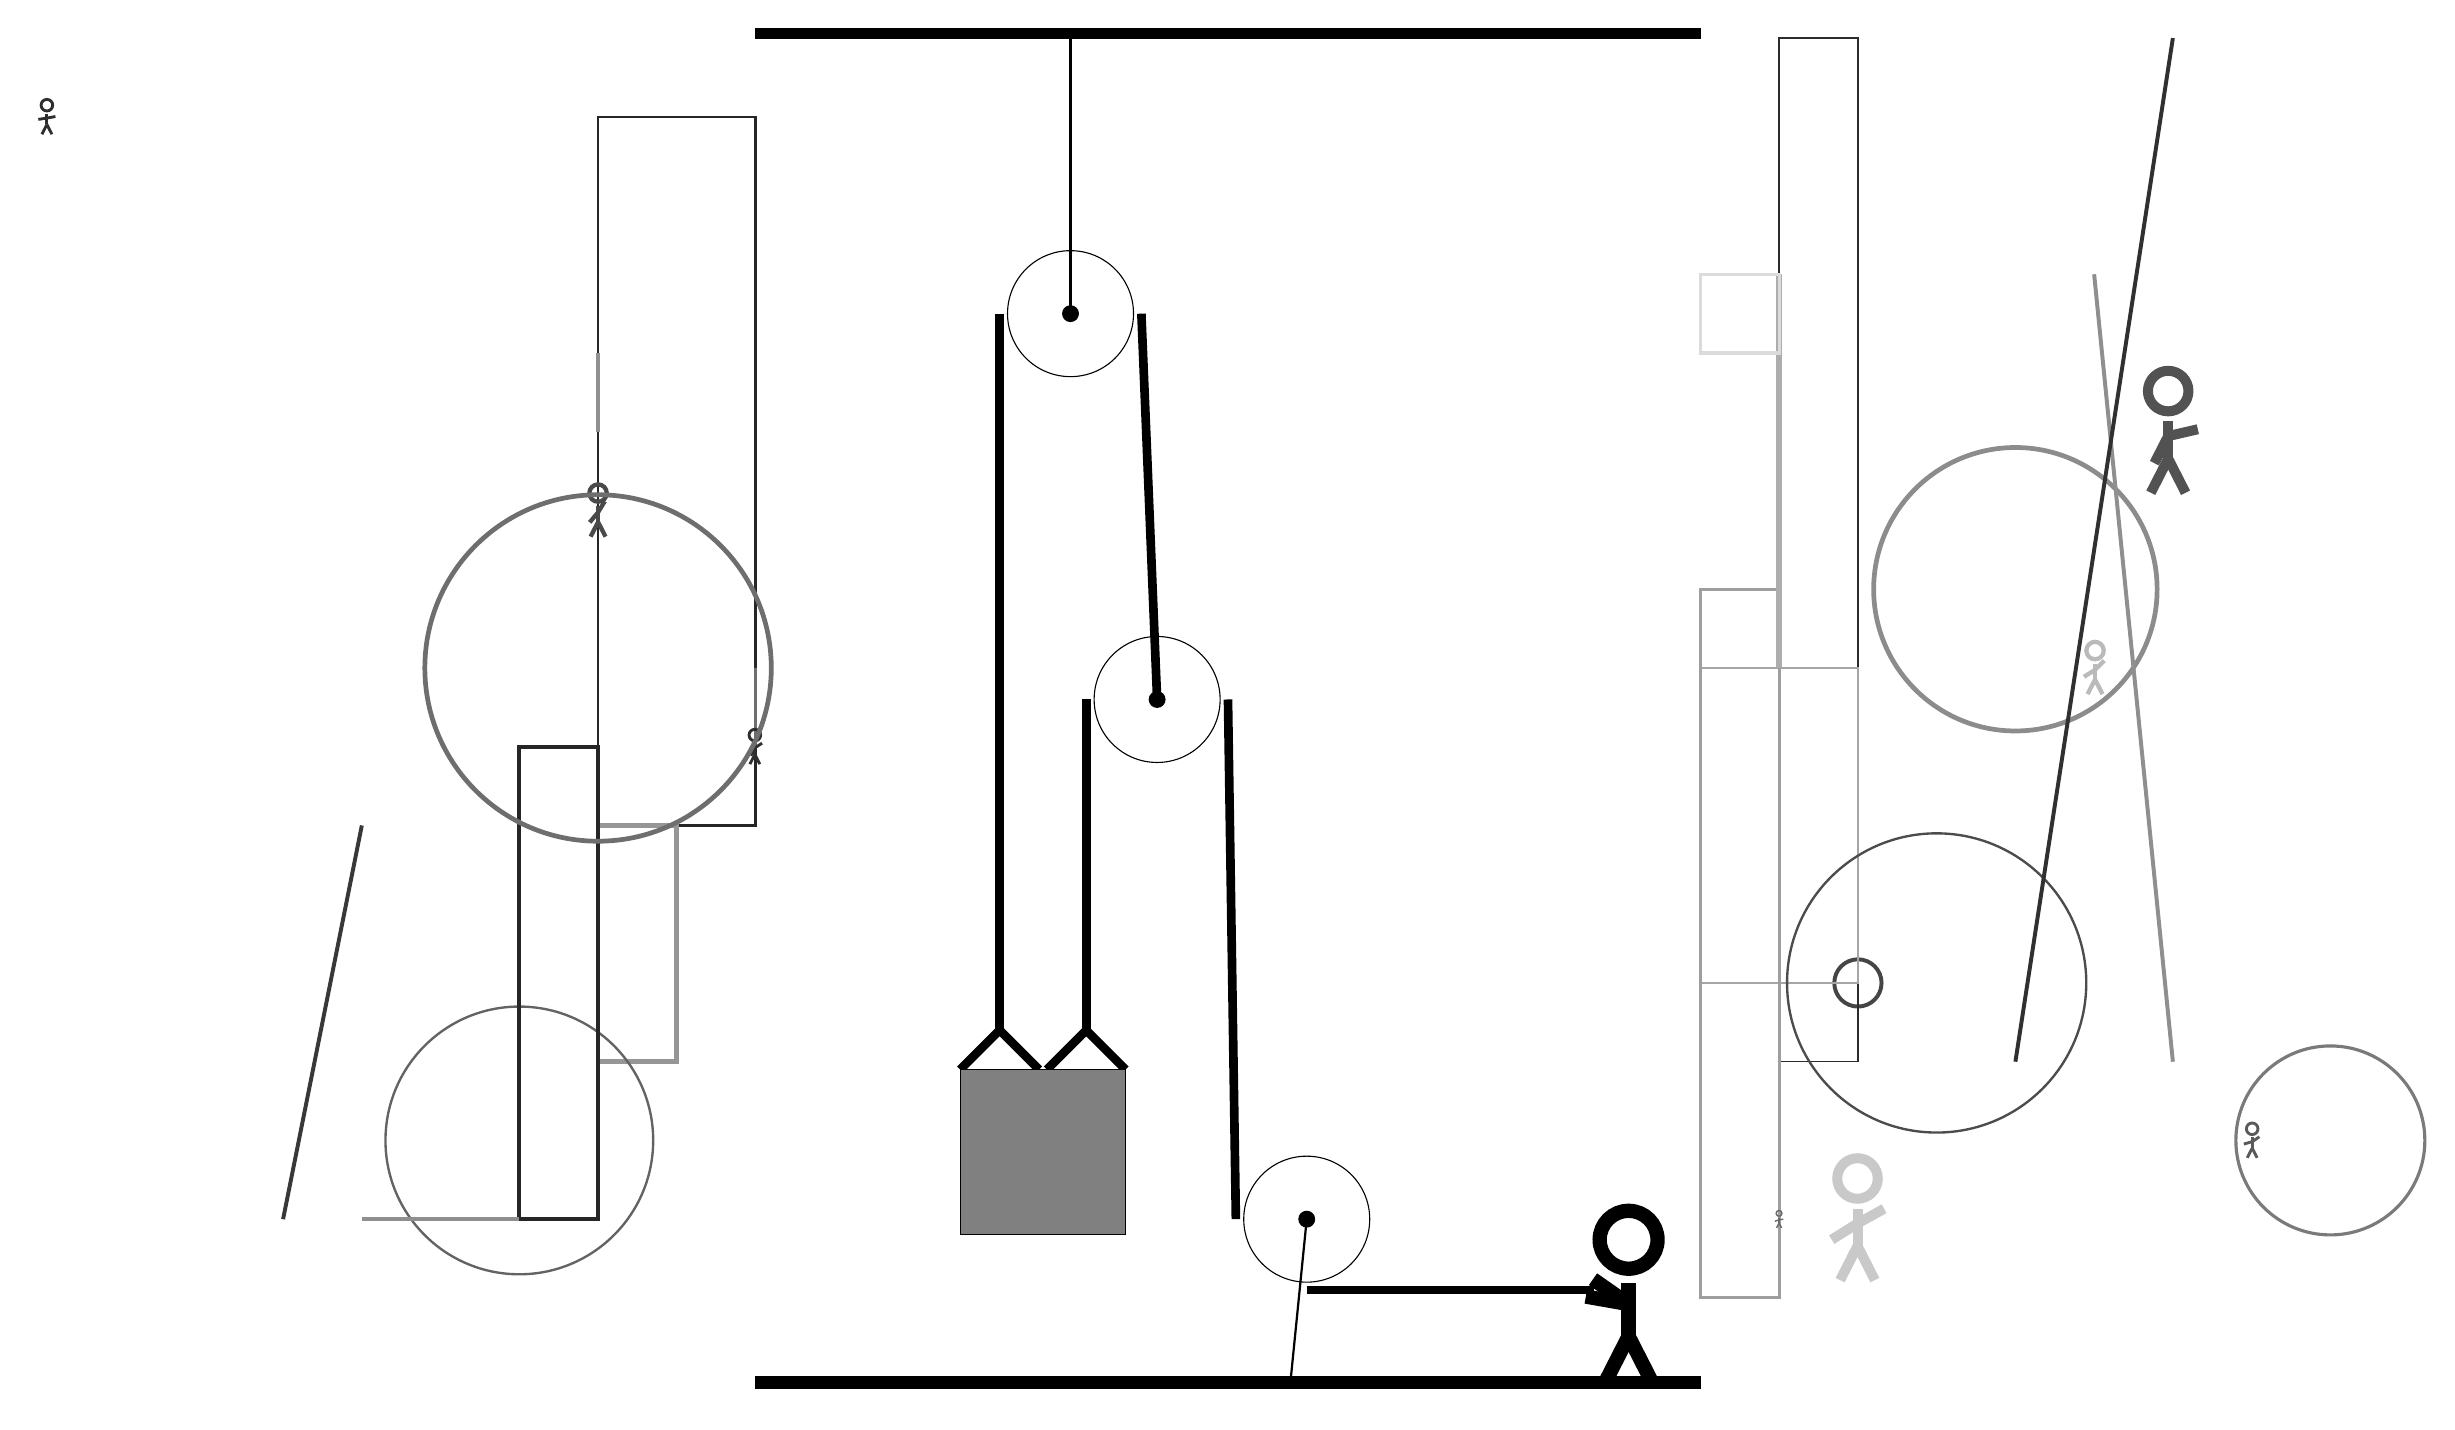
\begin{tikzpicture}
			%%%%% START %%%%%
			
			\draw[fill=black] (-2, 14) rectangle (10, 14.125);
			
			\draw (2, 10.5) circle (0.8);
			\draw[fill=black] (2, 10.5) circle (0.1);
			\draw[thick] (2, 10.5) -- (2, 14);
			
			\draw (3.1, 5.6) circle (0.8);
			\draw[fill=black] (3.1, 5.6) circle (0.1);
			
			\draw (5, -1) circle (0.8);
			\draw[fill=black] (5, -1) circle (0.1);
			\draw[thick] (5, -1) -- (4.8, -3);
			
			\draw[line width = 1.1mm]  (0.6, 0.9) -- (1.1, 1.4) -- (1.6, 0.9);
			\draw[line width = 1.1mm]  (1.7, 0.9) -- (2.2, 1.4) -- (2.7, 0.9);
			\draw[fill=black!50] (0.6, 0.9) rectangle (2.7, -1.2);
			
			\draw[line width = 1.1mm] (1.1, 10.5) -- (1.1, 1.4);
			\centerarc[line width = 1.1mm](2, 10.5)(0:180:0.9);
			\draw[line width = 1.1mm] (2.9, 10.5) -- (3.1, 5.6);
			\draw[line width = 1.1mm] (2.2, 5.6) -- (2.2, 1.4);
			\centerarc[line width = 1.1mm](3.1, 5.6)(0:180:0.9);
			\draw[line width = 1.1mm] (4.0, 5.6) -- (4.1, -1);
			\centerarc[line width = 1.1mm](5, -1)(180:270:0.9);
			\draw[line width = 1.1mm] (5, -1.9) -- (8.65, -1.9);
			
			\draw[line width=0.3mm, color=black!85] (-2, 4) rectangle (-4, 13);
			
			\draw [line width=0.5mm, color=black!73](12, 2) circle (0.3);
			\draw[line width=0.2mm, color=black!83] (11, 1) rectangle (12, 14);
			\draw[line width=0.3mm, color=black!35] (12, 6) rectangle (10, 2);
			\draw[line width=0.5mm, color=black!43](-4, 9) -- (-4, 10);
			
			\draw [line width=0.4mm, color=black!52](18, 0) circle (1.2);
			\draw[line width=0.4mm, color=black!57] (-2, 6) rectangle (-2, 5);
			\draw [line width=0.3mm, color=black!70](13, 2) circle (1.9);
			\draw[line width=0.6mm, color=black!41] (-3, 1) rectangle (-4, 4);
			
			\draw [line width=0.3mm, color=black!61](-5, 0) circle (1.7);
			
			\draw [line width=0.6mm, color=black!45](14, 7) circle (1.8);
			\node[line width=0.5mm, color=black!27] at (15, 6) {\Strichmaxerl[3][32][45]};
			\draw[line width=0.4mm, color=black!38] (11, 7) rectangle (10, -2);
			
			\node[line width=0.6mm, color=black!68] at (16, 9) {\Strichmaxerl[7][63][13]};
			\node[line width=0.3mm, color=black!71] at (-4, 8) {\Strichmaxerl[3][50][59]};
			\draw[line width=0.5mm, color=black!85] (-4, 5) rectangle (-5, -1);
			
			\node[line width=0.5mm, color=black!82] at (-2, 5) {\Strichmaxerl[2][63][34]};
			
			\draw[line width=0.7mm, color=black!32] (11, 6) rectangle (11, 11);
			\draw[line width=0.4mm, color=black!14] (11, 11) rectangle (10, 10);
			
			\draw[line width=0.5mm, color=black!44](-7, -1) -- (-5, -1);
			\node[line width=0.4mm, color=black!21] at (12, -1) {\Strichmaxerl[7][32][29]};
			
			\node[line width=0.5mm, color=black!58] at (11, -1) {\Strichmaxerl[1][20][7]};
			\node[line width=0.6mm, color=black!82] at (-11, 13) {\Strichmaxerl[2][9][10]};
			\draw[line width=0.5mm, color=black!78](-7, 4) -- (-8, -1);
			\draw[line width=0.5mm, color=black!44](15, 11) -- (16, 1);
			
			\draw [line width=0.6mm, color=black!57](-4, 6) circle (2.2);
			\draw[line width=0.5mm, color=black!81](14, 1) -- (16, 14);
			\node[line width=0.5mm, color=black!65] at (17, 0) {\Strichmaxerl[2][16][34]};
			
			\node at (9, -2) {\Strichmaxerl[10][-35][170]};
			
			\draw[fill=black] (-2, -3) rectangle (10, -3.15);
			
			%%%%% END %%%%%
		\end{tikzpicture}
	\end{figure}	
\end{document}